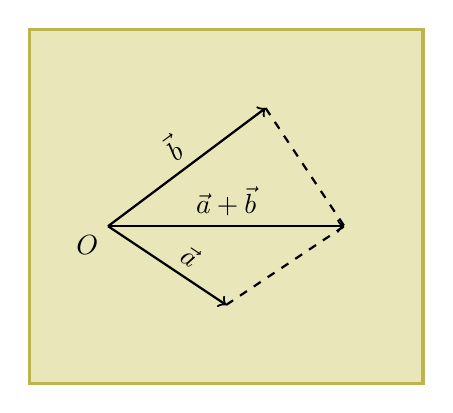
\begin{tikzpicture}
  \draw[draw = olive!60, fill = olive!20, very thick]
    (-1, -2) rectangle (4, 2.5);

  \draw[->, thick] (0, 0) -- (2, 1.5)
    node[midway, above, sloped] {\(\vec{b}\)};
  \draw[->, thick] (0, 0) -- (1.5, -1)
    node[pos = 0.6, above, sloped] {\(\vec{a}\)};
  \draw[->, thick] (0, 0) -- (3, 0)
    node[midway, above, sloped] {\(\vec{a} + \vec{b}\)};

  \draw[dashed, thick] (2, 1.5) -- (3, 0);
  \draw[dashed, thick] (1.5, -1) -- (3, 0);
  \draw (0, 0) node[below left] {\(O\)};
\end{tikzpicture}
